\section{Implementation and Microbenchmarks}
\label{sec:impl}

This section provides implementation details of our opportunistic GPU functions and microbenchmarks of the optimizations. 
We have implemented the scheduling and multiplexing policies as part of a control plane for hybrid serverless computing.
We use \sysname~\cite{fuerst2023iluvatar} as the base, and our implementation has has three main components: i) GPU scheduling policies, ii) CUDA multiplexing, and iii) policies for dispatching functions to both CPUs and GPUs based on speedup.
\sysname~is a low latency and highly scalable FaaS control plane whose overheads are more than 100x lower than OpenWhisk for CPU workloads, which it achieves due to per-worker queues, and asynchronous and batched execution of non-critical resource management operations. 
Our GPU function implementation adheres to the above design principles, and is implemented in around 3,000 lines of Rust. 

Invocations are dispatched by a dedicated thread which monitors available GPU resources, and if GPU tokens are available, selects a function to execute based on Algorithm~\ref{algo:dispatch} described in the previous section.
The dispatch thread is also notified upon invocation completion events, which helps maintain high device parallelism (\D). 
For servers with multiple GPUs, we maintain a single dispatcher which allows late binding of functions to individual GPUs.
Locality is still maintained by the dispatcher implementing \quotes{sticky} load balancing among GPUs: line~\ref{lst:line:in_flight} helps us avoid moving functions across GPUs and miss the high impact of cold-starts.
Function flows and \VT~tracking are kept in one data structure, and protected behind Read/Write locks. 

GPU functions have a special \quotes{Device} tag as part of their registration metadata, which also informs scheduling decisions.
GPU functions may also register a CPU counterpart, which is invoked when GPU acceleration is not necessary.
The CPU vs. GPU dispatch decision is made before functions are inserted into the respective device queues.
Our current dispatch policy creates and uses the GPU speedup as the key decision metric, and runs the top-p percentile of functions on GPUs (i.e., using a relative utility framework).
We have also implemented more advanced dispatch policies which consider multiple attributes like popularity and speedup, but we focus on the above simple static policy to keep the focus on the GPU scheduling. 


% Its integrated GPU shares a memory space with host CPU, so we cannot overcommit and migrate memory, limiting the GPU container pool.
%Even then, the fairness properties of \QName~and its hybrid CPU+GPU dispatching show similar benefits, and we elide them for space considerations.


\mhead{Utilization monitoring}
% Using t
We track both GPU compute utilization and per-container and total device physical memory usage.
Using NVML~\cite{nvml} bindings in Rust, we query compute utilization and record its instantaneous and moving average, for use in determining \D.
% Originally, we used the \emph{nvidia-smi}~\cite{nvidia-smi} CLI program for this, but found it took 1-2 seconds per update, caused high overhead, and was neither effective at tracking utilization nor easily parsable.
% If the updates are too infrequent, the platform will think more compute is available than reality, and over-schedule functions on a GPU.
% With NVML only taking roughly 100 $\mu{}s$, we query this information every 200 ms to balance having up-to-date information while avoiding excessive CPU utilization on the host.
We query this information every 200 ms to balance having up-to-date information while avoiding excessive CPU utilization on the host.
% The in-worker recored utilzation is also incremented on each dispatch by a factor of $1/D_{max}$ to avoid a thundering herd.
To track memory usage, our shim includes a report of memory allocations still held by the application to the worker alongside other invocation results. 
This data updates the container's record in the worker, which then tracks memory pressure on the device.
When a container needs to run, or a flow is made active, we can evict containers belonging to inactive flows. 
% , memory reporting, etc.


\begin{figure}
  \centering
  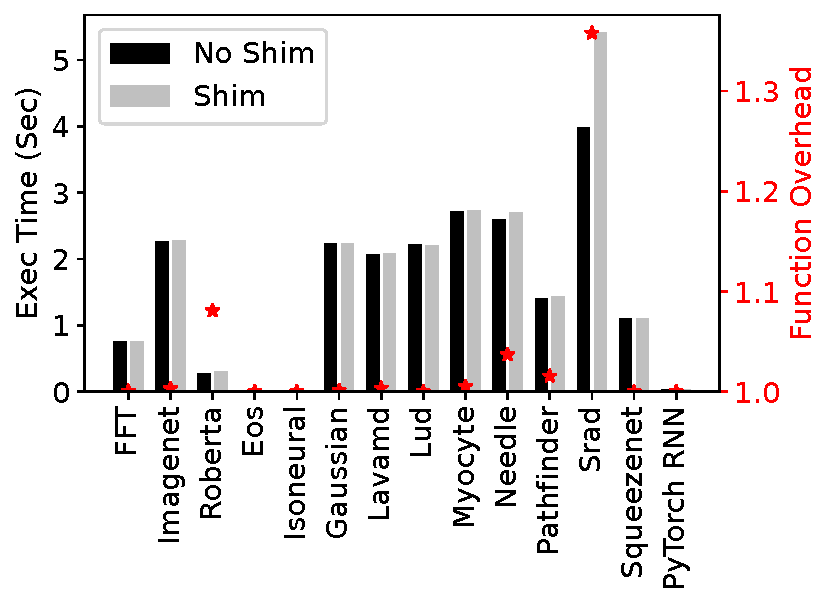
\includegraphics[width=0.7\textwidth]{./mqfq-final/graphs/driver-compare/8-exec_time.pdf}
  \caption{Functions see little to no impact from our interception and substitution of allocation calls.
          This matches performance promised by Nvidia for UVM applications.}
          \label{fig:shim-overhead}
\end{figure}


\subsection{CUDA Interposition Shim}
% Functions are run inside nvidia-docker \todo{any special changes?}.
We run functions inside Docker containers~\cite{docker-main} using the Nvidia Container Toolkit~\cite{nvidia-container} to attach specific GPUs to them. 
For dedicated GPUs with limited memory, we use a CUDA interposition ``shim'' which intercepts CUDA calls made by the function. 
Our shim implementation is similar to NVShare~\cite{alexopoulos2023nvshare}, but simpler: we only use it for intercepting memory allocation calls and forcing the function to use virtual memory.
This requires about 500 lines of code (written in C) to be injected using \funcname{LD\_PRELOAD}.
We use CUDA's Unified Virtual Memory (UVM) to oversubscribe device memory.
When using UVM, the application sees a unified host-device memory space, with memory pointers being valid in both spaces.
The CUDA driver moves and ensures coherency of UVM memory between the host and device as use and pressure demands, mimicking disk-based swap space found in operating systems.
Our shim intercepts all calls to the driver for allocations for physical memory made via \funcname{cuMemAlloc}, and makes a UVM allocation of the same size using \funcname{cuMemAllocManaged}.
We record the size and memory pointer position, then return the pointer to the application, thus maintaining  execution transparency. 
It can use this memory as if it were physically allocated, reading, writing, or copying it to the host using traditional driver calls. 
If the function already uses UVM, we intercept and forward its allocations, recording the metadata for our memory management tasks. 

The performance overhead of our interception is primarily influenced by the memory access patterns of the function and the extra layer of virtual memory (UVM), and is shown for different functions in Figure~\ref{fig:shim-overhead}. 
%We never adjust where the function's memory is, so any overhead will be caused by interceptions and usage of UVM allocations.
%Figure collates a variety of different function types and how they were affected.
All results are averaged over 10 trials, and we see a negligible latency impact on most functions. 
The rest see single-digit percentage increases, with \funcname{Srad} standing out with a 30\% overhead in execution time due to the UVM shim. 
These results are in line with Nvidia's own reporting on the performance change when migrating applications to UVM~\cite{nvidia-uvm}.
This low overhead shim is thus ideal for virtualizing GPU memory. 
%With our driver having such little impact, it is ideal for enabling a warm container pool of GPU containers and moving function memory off device when idle.

\begin{figure}
  \centering
  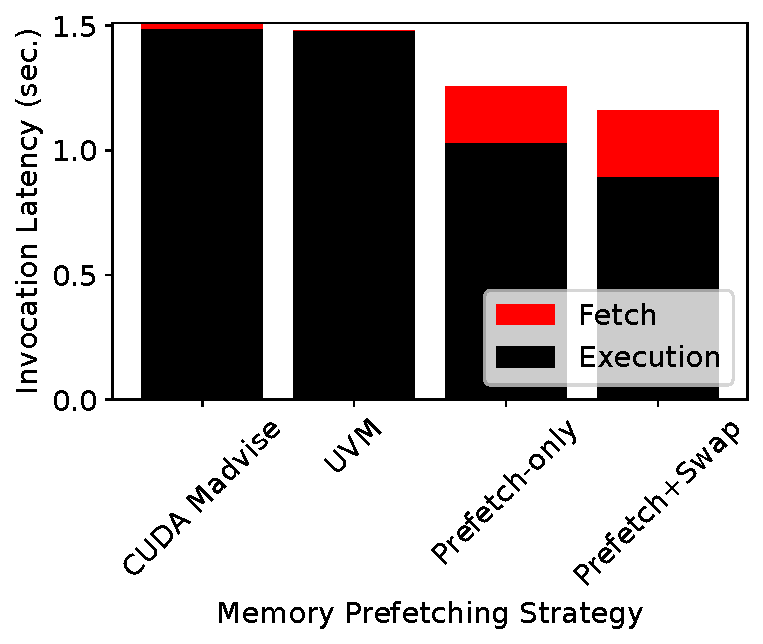
\includegraphics[width=0.6\textwidth]{./mqfq-final/graphs/mem-move/f16-i20-driver-mps-move.pdf}
  \caption{Active memory management (\texttt{Prefetch+Swap}) improves execution latency.}
  \label{fig:mem-prefetch}
% Fetch Strat, Exec Time, Fetch Time, Total Time
% Madvise 1.4893044978380203 0.021360369771718932 1.5106648676097392
% None 1.4704825393855572 1.2621283531188965e-06 1.4704838015139103
% Prefetch To 0.830518102645874 0.4062889523804188 1.2368070550262928
% Prefetch 0.7852441824972629 0.22023404985666276 1.0054782323539257
\end{figure}

\subsection{Memory Management}

We implement the warm pool, memory prefetching, and swapping optimizations inside the control plane, integrated with the scheduler. 
Recall that we prefetch the GPU memory of active functions, which is not provided out-of-the-box by CUDA UVM. 
% \texttt{madvise} (via \texttt{cuMemAdvise}). 
Default UVM only moves memory on-demand, and also exposes \texttt{madvise} hints (via \texttt{cuMemAdvise}) for memory ranges, but neither allow for deterministic control of memory placement.
Our default policy (\texttt{Prefetch+Swap}) asynchronously copies memory to the device before invocation, and swaps it back to host memory after the flow becomes idle (or evicted on-demand using a least recently used policy). 
After we choose a flow for dispatch, we call \funcname{cuMemPrefetchAsync} from the shim to prefetch the container's GPU memory.
% The prefetch driver call also is non-blocking, allowing us to rapidly call it on each allocation.
% allowing us to overlap the time it takes to prepare the memory
Doing this in a non-blocking manner allows us to overlap prefetching with the control plane marshalling invocation arguments to send to the container. 
Not having to block while waiting for memory to be moved saves significant time on the critical path.
% so we make this call and then send the invocation and its arguments to the container.
% Performing them in this order allows us to overlap this host-to-device memory movement with our platform actions.
When a flow is throttled or memory is needed to run other functions, we direct the shim to again use \funcname{cuMemPrefetchAsync} move memory off the device to CPU memory. 


We compare different memory management policies in Figure~\ref{fig:mem-prefetch}.
We run 16 copies of the FFT function from Table~\ref{tab:gpu-cpu}, each using 1.5 GB of device memory which oversubscribes the GPU's memory by 50\%. 
% To show the importance of locality of function memory and available space, we run 16 copies of the FFT function from Table~\ref{tab:fun-list}, each using 1.5 GB of device memory that, in aggregate, oversubscribe GPU memory by 50\%.
Each copy is sequentially invoked 20 times.
The impact of these different memory policies are displayed in Figure~\ref{fig:mem-prefetch}, with average time spent in-shim shown in red and function code execution in black.
With such high overcommttment and the stock UVM driver controlling data placement, the  execution time is 40\% worse than the optimal seen in Table~\ref{tab:gpu-cpu}.
Execution time is higher because memory must be paged in on-demand from the host as kernels access it, and old memory paged out.
% An intial proactive mechanism of telling the driver our data location preference, \texttt{Madvise}, tells the CUDA memory system we would prefer the memory onto the card, and after execution to prefer it off.
Surprisingly, using \texttt{CUDA Madvise} to control memory placement performs slightly worse. 
The madvise calls to the driver don't actually move any memory, and we just waste time sending the memory directives with no benefit to execution time. 
In contrast, our \texttt{Prefetch+Swap} policy reduces latency by over 33\% compared to stock UVM.
We also compare against a \texttt{Prefetch-only} policy which does not proactively swap function memory but instead relies on UVM for reclaiming pages. 
This shows that adding the swapping optimization (our default), provides a latency improvement 6\%, and matches the ideal non-UVM execution time listed in Table~\ref{tab:gpu-cpu}. 

Our system can also run on heterogeneous and edge hardware, such as the Nvidia Jetson Orin AGX. 
% Our implementation is expected to show similar trends on edge devices like Jetson Orin AGX\@.
% Jetson AGX Orin is a popular edge device with an integrated Ampere Architecture GPU~\cite{jetson-specs}.
% On this platform, iGPU (integrated GPU) use system memory and for a dGPU (discrete GPU) unified memory is not supported currently~\cite{tegra-uvm}.
Because its integrated GPU has no dedicated memory, our memory prefetching optimizations are not applicable, but all the other locality, fairness, and dispatching enhacements are relevant. 


%%% Local Variables:
%%% mode: latex
%%% TeX-master: "paper"
%%% End:
